\documentclass[13pt]{article}
\renewcommand{\baselinestretch}{1.0}
\usepackage[utf8]{vietnam}
\usepackage[a4paper, total={6in, 8in}]{geometry}
\usepackage[vietnamese,english]{babel}
\usepackage{hyperref}
\usepackage{mathtools}
\usepackage{amssymb}
\usepackage{indentfirst}
\usepackage{graphicx}
\usepackage{minted}
\usepackage{ragged2e}
\usepackage[nottoc]{tocbibind}

\hypersetup{
    colorlinks=true,
    linkcolor=blue,
    citecolor=blue,
    urlcolor=blue,
}
\begin{document}
\begin{titlepage}
    \begin{center}
        \vspace*{1.8cm}
        \Large
        Distributed System Labwork 1\\
        \Large
        \vspace{0.5cm}
        \begin{center}
            
\includegraphics[scale=1.0]{images/usth_logo1.PNG}
        \end{center}  
        \vspace{0.5cm}
            Group 1 - ICT\\
        \vspace{0.5cm}
            University of Science and Technology of Hanoi\\
        \vspace{0.5cm}
            January, 2022
        \vfill
          
   \end{center}
\end{titlepage}

\newpage
\tableofcontents
\newpage

\section{Introduction}
\subsection{Overview}
\noindent%
In this labwork, we try to build a file transfer over TCP/IP in CLI, based on the
provided chat system.

\subsection{Protocol}

\begin{figure}[h]
    \centering
    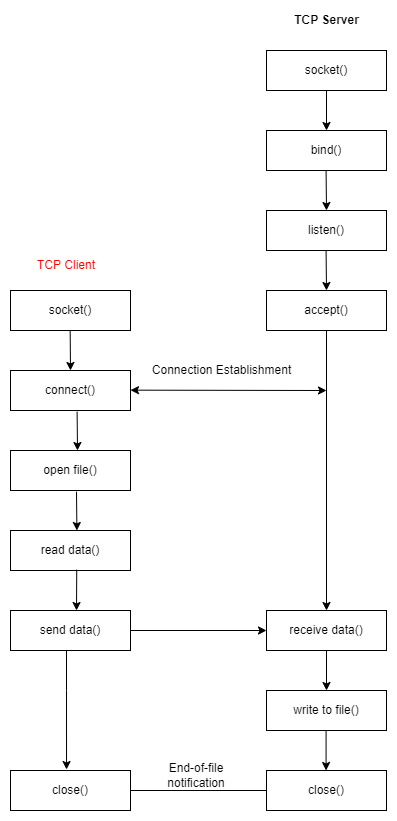
\includegraphics[scale=0.5]{images/tcp.drawio.png}
    \caption{Protocol diagram}
    \label{fig:protocol}
\end{figure}

\subsection{System organization}
\noindent%
The server creates a specific port, for eg: 9819. From the client CLI, it takes 2 arguments, IP address and the port to connect to the server. One client connects to one server only. The client send data through a character array called buffer. The buffer has a maximum length of 255. After receiving the buffer, the server will writes it to the file. The client will notice the server there is nothing left after reaching end-of-file. Afterwards, both server and client will close.

\begin{figure}[H]
    \centering
    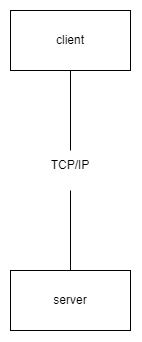
\includegraphics[scale=1.0]{images/system.png}
    \caption{System organization}
\end{figure}

\subsection{Implementation}
\noindent%
We have implemented the client side:

\begin{minted}{c}
#include <unistd.h>
#include <stdio.h>
#include <sys/socket.h>
#include <stdlib.h>
#include <netinet/in.h>
#include <string.h>
#include <netdb.h>
void error(const char* msg) {
	//print system error message
	perror(msg);
	exit(1);
}

void send_file(FILE* f, int sockfd) {
	char buffer[1024] = { 0 };
	while (fgets(buffer, sizeof(buffer), f) != NULL) {
		int i = send(sockfd, buffer, sizeof(buffer), 0);
		if (i == -1) {
			error("Error in sending data");
		}
		memset(&buffer, 0, sizeof(buffer));

	}
}


int main(int argc, char* argv[]) {
	int so;
	char s[100];
	struct sockaddr_in ad;


	socklen_t ad_length = sizeof(ad);
	struct hostent* hep;

	// create socket
	int serv = socket(AF_INET, SOCK_STREAM, 0);

	// init address
	hep = gethostbyname(argv[1]);
	memset(&ad, 0, sizeof(ad));
	ad.sin_family = AF_INET;
	ad.sin_addr = *(struct in_addr*)hep->h_addr_list[0];
	ad.sin_port = htons(12345);

	// connect to server
	connect(serv, (struct sockaddr*)&ad, ad_length);

	memset(&s, 0, 100);
	FILE* f;
	f = fopen("send.txt", "r");
	if (f == NULL) {
		error("Error in reading file.");
	}
	else {
		printf("Reading file successfully..\n");
	}
	rewind(f);
	send_file(f, serv);
	printf("The file has been transfered successfully...\n");
	printf("Close...\n");
	close(serv);
	return 0;


}

\end{minted}
\noindent%
We have implemented the server side:
\begin{minted}{c}
#include <unistd.h>
#include <stdio.h>
#include <sys/socket.h>
#include <stdlib.h>
#include <netinet/in.h>
#include <string.h>

void error(const char* msg) {
	//print system error message
	perror(msg);
	exit(1);
}

void write_file(FILE* fp, int sockfd) {
	char buffer[1024];

	while (1) {
		int n = recv(sockfd, buffer, sizeof(buffer), 0);
		if (n <= 0) {
			break;
		}
		fprintf(fp, "%s", buffer);
		memset(&buffer, 0, sizeof(buffer));
	}
	return;

}

int main() {
	int ss, cli, pid;
	struct sockaddr_in ad;
	char s[100];
	socklen_t ad_length = sizeof(ad);
	FILE* fp;
	// create the socket
	ss = socket(AF_INET, SOCK_STREAM, 0);

	// bind the socket to port 12345
	memset(&ad, 0, sizeof(ad));
	ad.sin_family = AF_INET;
	ad.sin_addr.s_addr = INADDR_ANY;
	ad.sin_port = htons(12345);
	bind(ss, (struct sockaddr*)&ad, ad_length);

	// then listen
	listen(ss, 0);

	while (1) {
		// an incoming connection
		cli = accept(ss, (struct sockaddr*)&ad, &ad_length);

		pid = fork();
		if (pid == 0) {
			printf("client connected\n");

			fp = fopen("received.txt", "w");
			if (fp == NULL) {
				error("Error in reading file.");
			}
			else {
				printf("Reading file successfully..\n");
			}
			write_file(fp, cli);
			printf("Received file.");

			return 0;
		}
		else {
			// continue the loop to accept more clients
			continue;
		}
	}

	// disconnect
	close(cli);
	close(ss);

}
\end{minted}
\subsection{Contribution}
\noindent%
\begin{table}[ht!]
  \begin{center}
    \label{tab:table1}
    \begin{tabular}{l|l}
      \textbf{Member} & \textbf{Contribution}\\
      \hline
      Nguyen Xuan Tung & Client code\\
      Nguyen Quang Anh & Server code\\
      Lu Khanh Huyen & Design Protocol\\
      Tran Hong Quan & Design Architecture\\
      Vu Duc Chinh & Report\\
    \end{tabular}
    \caption{Contribution Table}
  \end{center}
\end{table}


\end{document}
